\documentclass{article}
\usepackage{CJKutf8}
\usepackage{graphicx}
\title{零钱找零:动态规划}
\author{Ngoo Ling Hui}
\begin{document}
\begin{CJK*}{UTF8}{gbsn}
\maketitle

\section{算法分析}
这个算法解决的问题是动态规划中的零钱兑换问题,其目标是找出凑成特定金额所需的最小硬币数。以下是算法的主要思路:

\begin{itemize}
    \item 动态规划数组: 创建一个一维动态规划数组 $dp$,其中$dp[i]$ 表示凑成金额 i 所需的最小硬币数。数组初始化为一个较大的值(例如 $INT\_MAX$),表示初始状态为无法凑成。
    \item 状态转移: 遍历硬币面额数组,对每个硬币进行状态转移。对于每个硬币面额 coin,从 coin 开始遍历到目标金额 amount,更新 $dp[j]$ 的值。状态转移方程为 $dp[j] = min(dp[j], dp[j - coin] + 1)$,表示选择硬币 coin 或不选择硬币 coin 中的最小值。
    \item 初始条件: 初始化 $dp[0]$ 为0,因为凑成金额0不需要任何硬币。
    \item 遍历所有硬币和金额: 使用两层嵌套循环,外层遍历硬币数组,内层遍历金额。
    \item 最终结果: 返回 $dp[amount]$ 的值,即凑成目标金额所需的最小硬币数。如果 $dp[amount]$ 仍然是初始值(未被更新),表示无法凑成目标金额,返回 -1。
\end{itemize}

这个算法的关键在于动态规划数组的设计和状态转移方程的建立。通过遍历硬币面额和金额,不断更新动态规划数组,最终得到的 $dp[amount]$ 就是问题的解。

\section{实验结果}
对于目标金额为 63 美分,硬币面额为 {1, 5, 10, 25} 的测试结果:
\begin{figure}
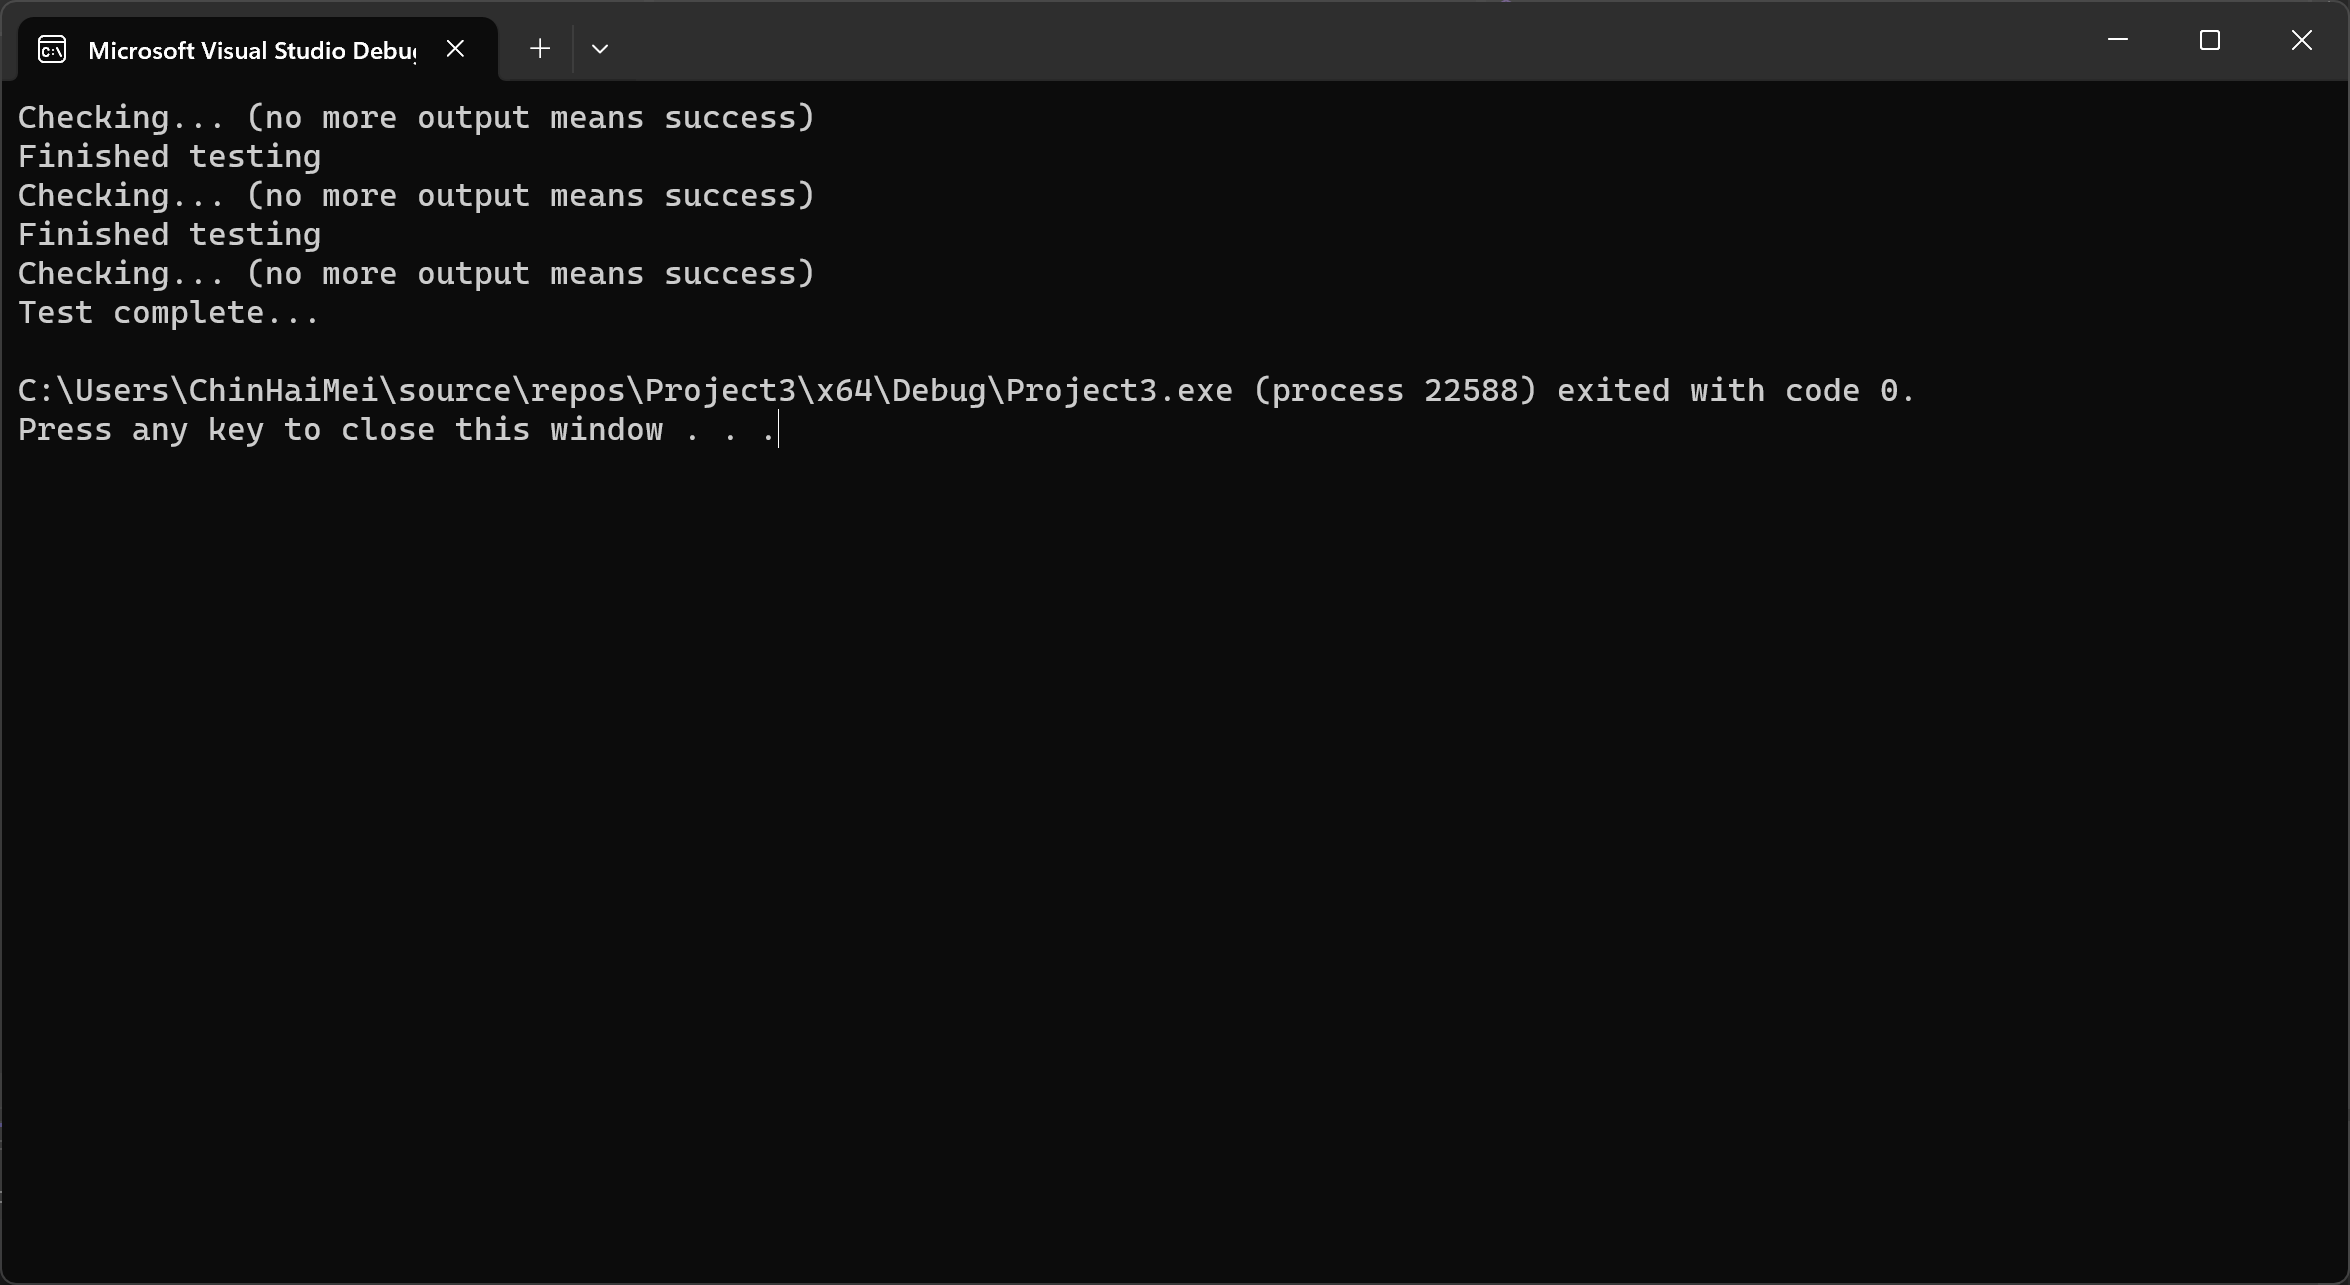
\includegraphics[width=0.5\textwidth]{image.png}
\end{figure}

\end{CJK*}
\end{document}
